\chap{Enhanced Generative Adversarial Network}

\section{Introduction}

\section{GAN Architecture} 

The original paper's\cite{Original-GAN} generator architecture consisted of  rectifier linear\cite{RELU} and sigmoid activations, while the discriminator net used maxout [10] activations. the results were good but lacked stability and also suffered from problem of model collapse.
Later, Radford \textit{et al.}\cite{DCGAN} proposed deep convolution generative adversarial network which used deep convolution with fractional stride convolution and batch normalization to stabilize the model. This work is uses this architecture as base and later adding conditional vector to it. The figure 4.1 shows the architecture of generator and discriminator. In this work, we use RELU
in all the layers expect the output. Since the paper Radford \textit{et al.}\cite{DCGAN} showed that that these can help in convergence of the model and it also covers the color space of the distribution.
\par

As you can see it figure the architecture of generator and discriminatory are exactly opposite to each other. The generator use up-convolution or commonly known as backward convolution to generate image.%J. Long, E. Shelhamer, and T. Darrell, “Fully convolutional networks for semantic segmentation,”CoRR, vol. abs/1411.4038, 2014. [Online]. Available: http://arxiv.org/abs/1411.4038
The discriminator is a standard deep convolution neural network used for classification of real or fake image
\begin{figure}
  \centering
    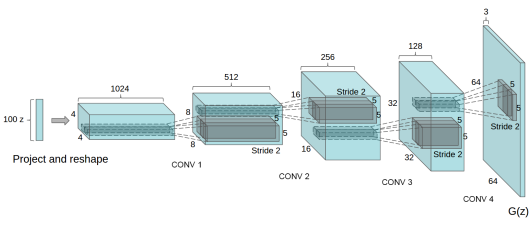
\includegraphics[scale=.7, angle=0]{Files/Generator-Architecture.png}
    \caption[Generator Architecture]{Generator Architecture\cite{DCGAN}}
    \label{fig: DCGAN}
\end{figure}

\section{Training GAN}

Training a GAN is always a tricky part. This work uses DCGAN\cite{DCGAN} as baseline. Since the DCGAN stabalizes the networks to a great extent. The major contribution of the DCGAN in our work is the use Batch-Normalization, strided convolution and ADAM optimizer. We will go through each of these steps one by one.
\subsection{BatchNomalization}

Batch Normalization for first introduced by Ioffe\textit{et al.}\cite{BatchNorm}. It was major landmark in area of deep learning as most deep neural network today's contains batch normalization. 
To understand batch normalization, we need to understand the problem it is trying to solve. It helps in minimizing internal co-variance shift. Internal covariate shift refers to change in input distribution. Since neural network are designed in hierarchical fashion, so even small changes can get amplified as we are dealing generally more than million parameters. To rectify this problem we normalise each batch at every layer by both mean and variance commonly known as whitning. The major advantage of the batch normalization are follows
\begin{itemize}
    \item Initial value of weights have less impact of gradient descent.
    \item It helps in keeping higher learning rate and accuracy. So it reduces overall training time and this helps in faster training of GANs.
\end{itemize}

\subsection{Strided Convolution}

The concept of deconvolution was first introduced by Zeiler \textit{et al} \cite{Deconv}. It also is commonly known as  strided convolution, transposed fractional convolution or upsampling.



\par
It basically is going from output of some convolution to the input to that convolution.For instance it is going from green matrix to the blue matrix as shown in below figure. So given a kernel K, the type of convoution is defined by how forward or backward passes are calculated\cite{Deconv-Theano}.

\begin{figure}
  \centering
    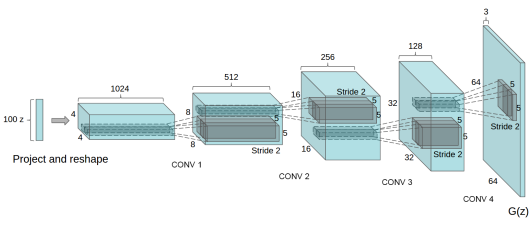
\includegraphics[scale=.7, angle=0]{Files/Generator-Architecture.png}
    \caption[Generator Architecture]{Generator Architecture\cite{DCGAN}}
    \label{fig: Simple-Conv}
\end{figure}

\begin{figure}
  \centering
    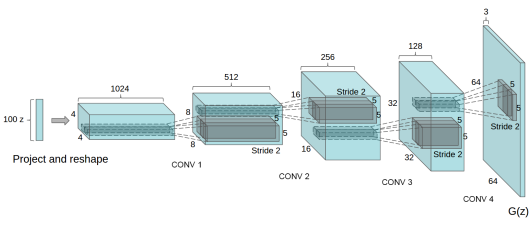
\includegraphics[scale=.7, angle=0]{Files/Generator-Architecture.png}
    \caption[Generator Architecture]{Generator Architecture\cite{DCGAN}}
    \label{fig: DCGAN}
\end{figure}
\begin{algorithm}[ht]
\caption{Learning a single layer, l, of the Deconvolutional\cite{Deconv}}
\label{alg:algorithm1}

\begin{algorithmic}[1]
\Require
    \Statex Training images y, \# feature maps K, connectivity g. \Statex Regularization weight $\lambda$, \# epochs E
    \Statex Continuation parameters: $\beta_0, \beta_Inc,\beta_Max $
\State Initialize feature maps and filters $z \sim N (0, \epsilon), f \sim N (0, \epsilon)$
\For {epoch in 1 to E}
    \For{i in 1 to I}
        \State$\beta=\beta_0$
        \While{$\beta <\beta_max$}
        \State $x^{i}_{k,l}= max(\left | z^{i}_{k,i} \right |-\frac{1}{\beta} ,0)\frac{z^{i}_{k,i}}{\left | z^{i}_{k,i} \right|}$
        \State $Z^{i}_{k,l}= max(\left | z^{i}_{k,i} \right |-\frac{1}{\beta} ,0)\frac{z^{i}_{k,i}}{\left | z^{i}_{k,i} \right|}$
        \EndWhile
    \EndFor
\EndFor
\end{algorithmic}
\end{algorithm}
